% ===============================
%          Chapter 2A.1
%         Cell Membranes
%     Created by Michael Tang
%           2025.02.14
% ===============================

\subsubsection{2A.1 Cell Membranes}
\paragraph{Cell Membranes and Their Functions}
\begin{itemize}
    \item \textbf{Cell Membrane:} Forms the outer boundary of a cell, controlling what enters and exits.
    \item \textbf{Membranes in Cells:} Found around \underline{organelles} \footnote{\textbf{Organelle:} An organelle is a
    specialized structure within a cell that performs a specific function. Examples include the nucleus (with contains genetic
    material), mitochondria (which produce energy), and the \underline{endoplasmic reticulum} (内质网, which hepls in protein and
    lipid synthesis). Organelles are often surrounded by membranes to \underline{compartmentalize} (划分) their functions within
    the cell.} (细胞器) like the nucleus and \underline{mitochondria} (线粒体).
    \item \textbf{Functions of Cell Membranes}
    \begin{itemize}
        \item Act as barriers, maintaining different conditions inside and outside the cell.
        \item Hold enzymes for reactions (e.g., respiration in mitochondria).
        \item Allow \underline{vesicles} (囊泡) to transport and secrete substances.
    \end{itemize}
\end{itemize}

\paragraph{The Structure of Membranes}
\begin{itemize}
    \item Composed of \underline{phospholipids} (磷脂) and proteins arranged in a specific way.
    \item \textbf{\underline{Phospholipid Bilayer} (磷酸双分子层)}
    \begin{itemize}
        \item \textbf{Phospholipid Molecule:}
        \begin{itemize}
            \item \textbf{\underline{Hydrophilic head} (亲水头):} Attracted to water, faces outwards.
            \item \textbf{\underline{Hydrophobic tail} (疏水尾):} Repelled by water, faces inwards.
        \end{itemize}
        \begin{figure}[H]
            \centering
            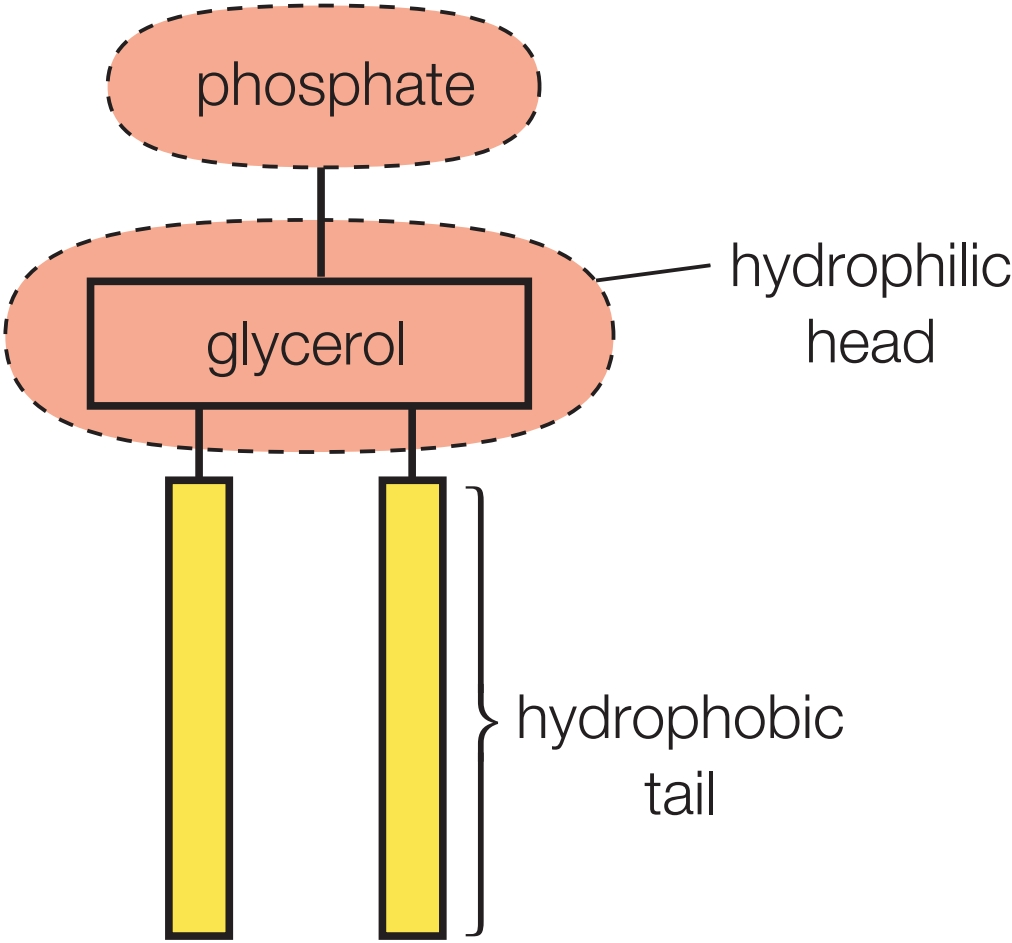
\includegraphics[scale=0.12]{Biology/2A/Images/2A-1-1.png}
            \caption{A phospholipid molecule.}
        \end{figure}
        \item In water, phospholipids self-assemble:
        \begin{itemize}
            \item \textbf{\underline{Monolayer} (单分子层):} At air / water interface.
            \item \textbf{\underline{Bilayer} (双分子层):} Hydrophilic heads outward, hydrophobic tails inward.
            \item \textbf{\underline{Micelle} (胶束):} Spherical structure in water.
        \end{itemize}
        \begin{figure}[H]
            \centering
            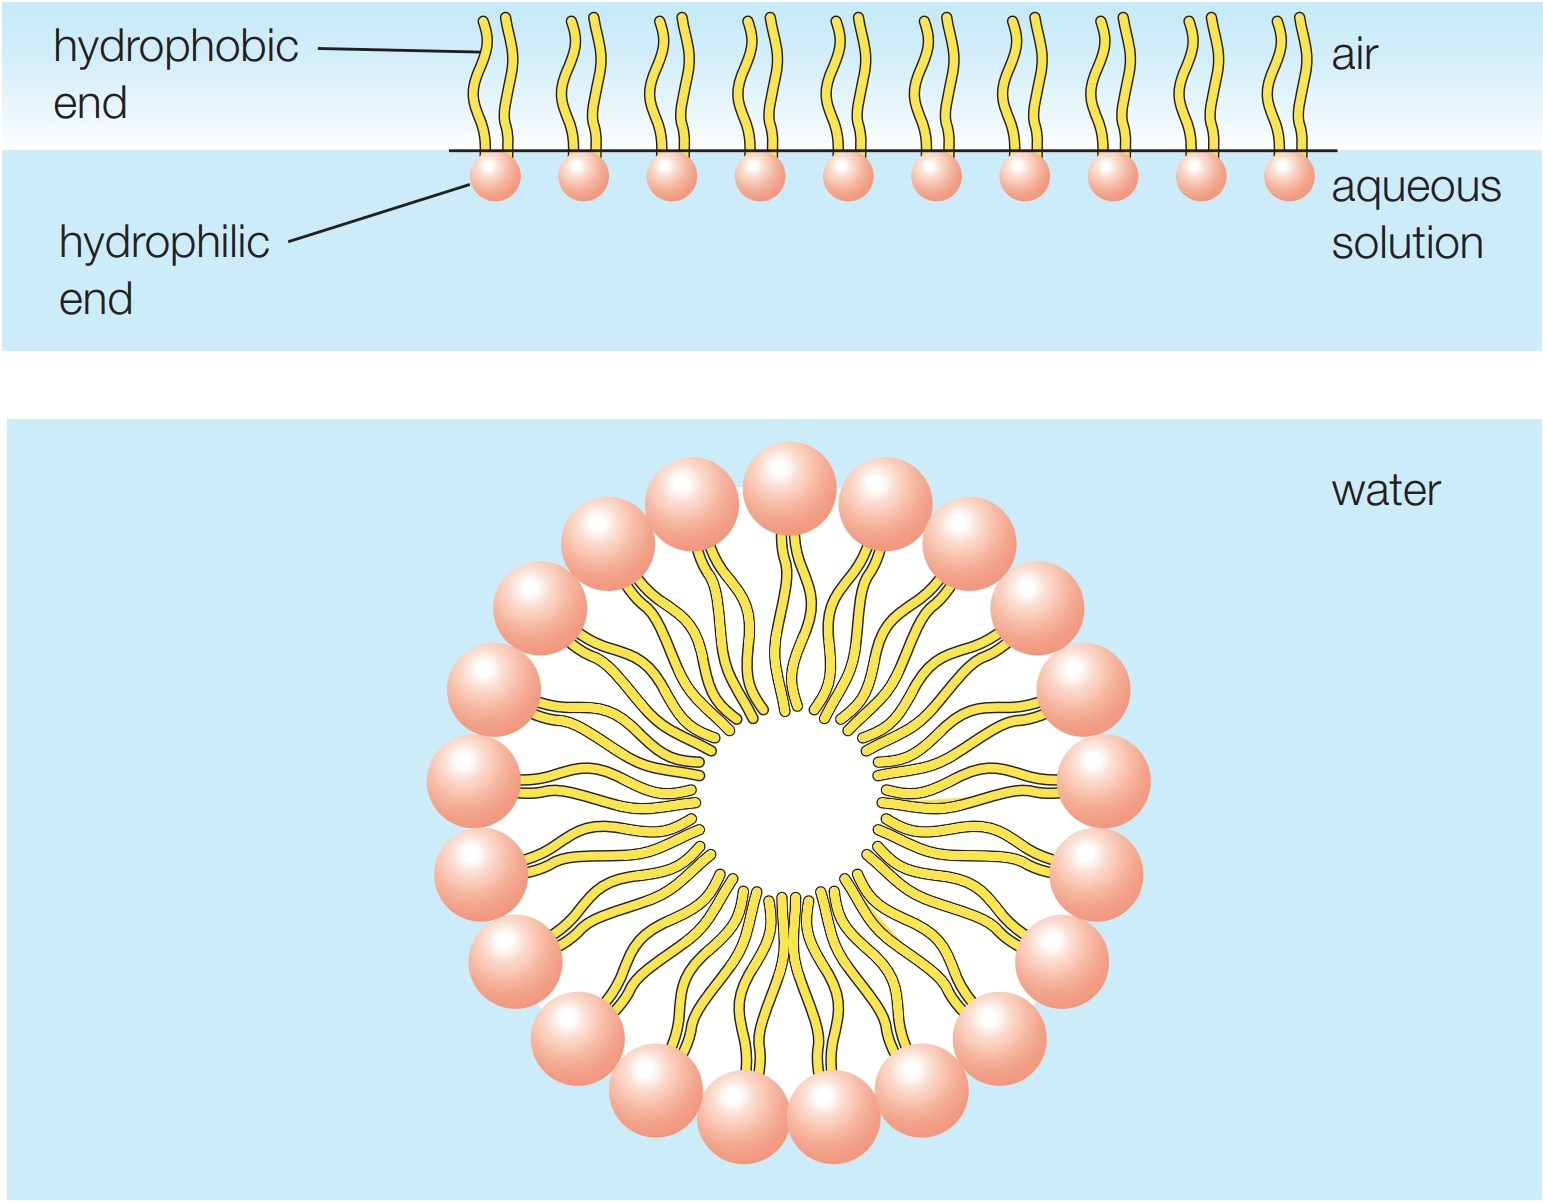
\includegraphics[scale=0.12]{Biology/2A/Images/2A-1-2.png}
            \caption{Phospholipids form a monolayer at an air / water junction and a micelle when water surrounds them.}
        \end{figure}
    \end{itemize}
    \item \textbf{Properties of the Bilayer}
    \begin{itemize}
        \item Acts as a barrier to most molecules.
        \item Allows fat-soluble molecules to pass but not ions.
        \item More fluid with unsaturated fatty acids.
        \item Cholestrol makes the membrane stronger and less \underline{permeable} (渗透性).
    \end{itemize}
\end{itemize}

\paragraph{\underline{The Fluid Mosaic Model} (流动镶嵌模型)}
\begin{itemize}
    \item Proposed by S. J. Singer and G. Nicolson in 1972.
    \item Membrane is dynamic, not rigid.
    \item Proteins float inthe lipid bilayer.
    \begin{itemize}
        \item \underline{Integral proteins} (整合蛋白) span the membrane.
        \item \underline{Peripheral proteins} (外周蛋白) are attached to the surface.
        \item \underline{Glycoproteins} (糖蛋白) help in cell recognition.
    \end{itemize}
    \begin{figure}[H]
        \centering
        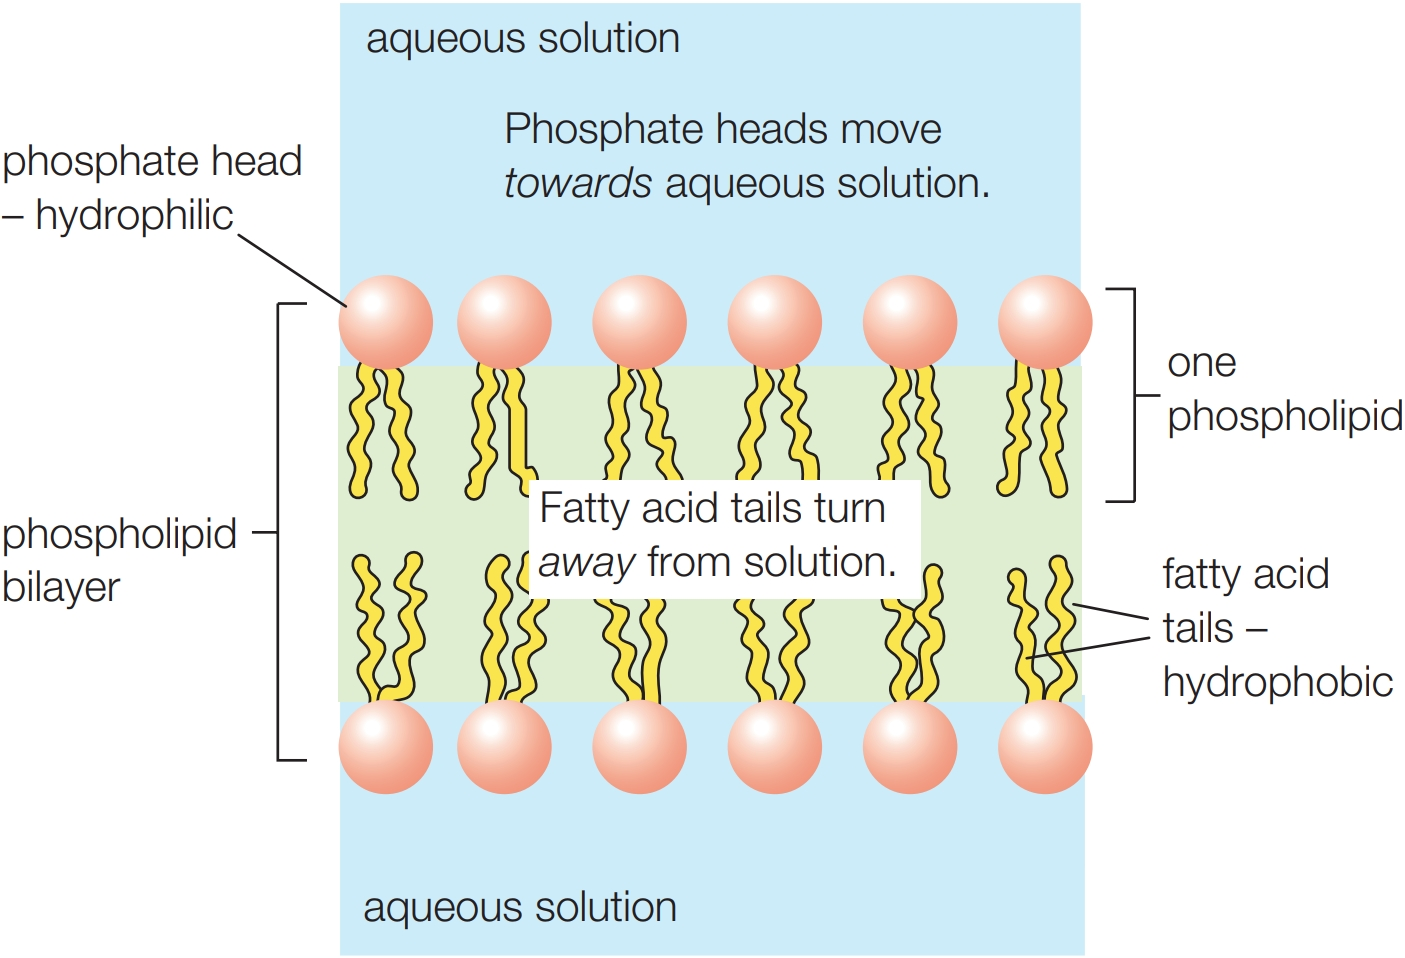
\includegraphics[scale=0.15]{Biology/2A/Images/2A-1-3.png}
        \caption{Phospholipids form a monolayer at an air / water junction and a micelle when water surrounds them.}
    \end{figure}
    \item \textbf{Functions of Membrane Proteins}
    \begin{itemize}
        \item \textbf{Transport:} Gated channels allow specific molecules through.
        \item \textbf{\underline{Receptors} (受体):} Detect hormones / signals.
        \item \textbf{Enzymes:} Speed up reactions.
        \item \textbf{Glycoproteins:} Involved in cell recognition.
    \end{itemize}
\end{itemize}

\paragraph{Scientific Models of Membranes}
\begin{itemize}
    \item Early experiments showed membranes contained lipids.
    \item 1935: \underline{Davson-Danielli Model} (达夫森-丹尼利模型) - Membrane had a lipid core with a protein layer.
    \item 1950s: \underline{Electron Microscopy} (电子显微镜) confirmed a bilayer.
    \item 1972: \underline{Fluid Mosaic Model} (流动镶嵌模型) replaced older models after further studies.
    \begin{figure}[H]
        \centering
        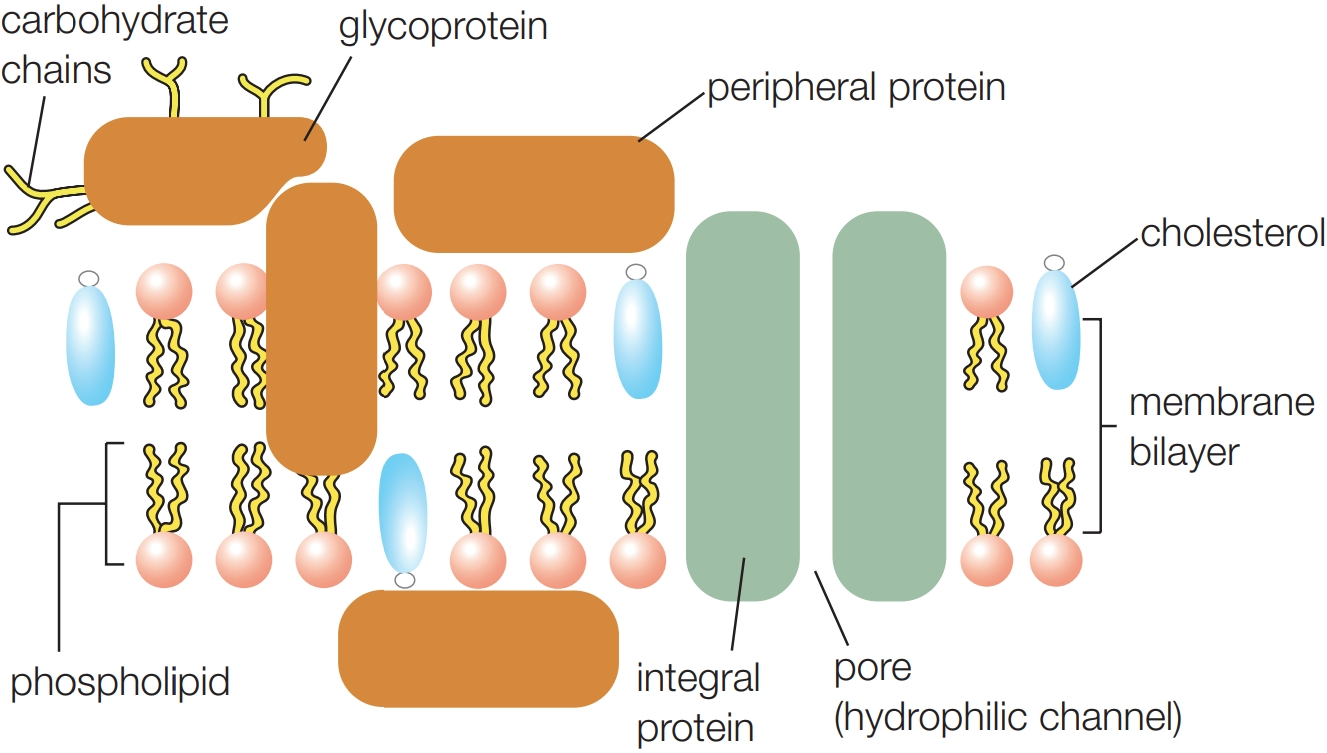
\includegraphics[scale=0.18]{Biology/2A/Images/2A-1-4.png}
        \caption{The fluid mosaic model of the cell membrane - a phospholipid sea with associated proteins, which may be floating
        or anchored within the membrane.}
    \end{figure}
\end{itemize}

\paragraph{Investigating Membrane Properties}
\begin{itemize}
    \item \underline{Red beet experiments} (红甜菜实验): More red \underline{dye} (染料) in water = more permeable membrane.
    \item Alcohol dissolves lipids, increasing permeability.
    \item High temperature \underline{denatures} (变性) proteins, making membranes leaky.
\end{itemize}

\paragraph{Exam Keys}
\begin{itemize}
    \item Phospholipid bilayer = barrier, but proteins control permeability.
    \item Membranes are flexible and fluid, not rigid.
    \item Cholesterol increases strength and reduces permeability.
    \item Use experimental data to explain membrane permeability changes.
\end{itemize}